\documentclass[aspectratio=169,11pt]{beamer}
\usepackage[T1]{fontenc}
\usepackage{lmodern}
\usepackage{amsmath,amssymb,mathtools}
\usepackage{booktabs}
\usepackage{tikz}
\usepackage{listings}
\usepackage{graphicx}
\usepackage{xcolor}
\usetikzlibrary{arrows.meta,positioning}
\definecolor{ink}{HTML}{17212B}
\definecolor{muted}{HTML}{566473}
\definecolor{accent}{HTML}{175B72}
\definecolor{warm}{HTML}{A34E2E}
\definecolor{pale}{HTML}{F5F7F8}
\setbeamercolor{normal text}{fg=ink,bg=white}
\setbeamercolor{frametitle}{fg=ink,bg=white}
\setbeamercolor{structure}{fg=accent}
\setbeamercolor{alerted text}{fg=warm}
\setbeamerfont{frametitle}{size=\Large,series=\bfseries}
\setbeamersize{text margin left=0.75cm,text margin right=0.75cm}
\setbeamertemplate{navigation symbols}{}
\setbeamertemplate{footline}{\hfill\color{muted}\scriptsize Acemoglu--Restrepo (2017) \quad \insertframenumber/\inserttotalframenumber\hspace{0.55cm}\vspace{0.22cm}}
\setbeamertemplate{itemize item}{\color{accent}$\blacktriangleright$}
\setlength{\parskip}{0.35em}
\newcommand{\key}[1]{{\color{accent}\bfseries #1}}
\newcommand{\sourcefoot}{\vfill{\color{muted}\scriptsize Source: Acemoglu and Restrepo, NBER WP 22252, revised June 2017.}}
\lstset{basicstyle=\ttfamily\scriptsize,columns=fullflexible,keepspaces=true,aboveskip=0pt,belowskip=0pt,frame=single,backgroundcolor=\color{pale},rulecolor=\color{muted},breaklines=true,showstringspaces=false,literate={ℝ}{{$\mathbb R$}}1 {∀}{{$\forall$}}1 {→}{{$\to$}}1 {γ}{{$\gamma$}}1 {₀}{{$_0$}}1 {Λ}{{$\Lambda$}}1 {σ}{{$\sigma$}}1 {ε}{{$\varepsilon$}}1 {≤}{{$\le$}}1 {∧}{{$\wedge$}}1}
\title{The Race Between Machine and Man}
\subtitle{Tasks, displacement, reinstatement, and what Lean actually checks}
\author{Gabriel Saco}
\date{24 September 2026}
\begin{document}

\begin{frame}
\titlepage
\vspace{-1.2em}
\centering\small Repository: \href{https://github.com/gsaco/ai-06-restrepo}{\texttt{github.com/gsaco/ai-06-restrepo}}
\end{frame}

\begin{frame}{Why the unit of analysis changes}
\large This paper asks how automation and new tasks jointly affect \key{aggregate} output, wages, factor shares, and employment.
\vspace{0.7em}
\begin{itemize}\setlength\itemsep{0.7em}
\item Earlier term papers center on a decision by an individual agent.
\item Here the outcome comes from equilibrium across \key{firms, households, capital markets, and innovation}.
\item A wage response cannot be read from one task: displaced workers move into the remaining labor tasks, while output and capital adjust.
\end{itemize}
\sourcefoot
\end{frame}

\begin{frame}{Three decisions form the economic problem}
\begin{columns}[T,onlytextwidth]
\column{0.31\textwidth}\key{Firms}\\[0.35em]Choose the lower unit cost in each feasible task; competitive prices equal costs.
\column{0.31\textwidth}\key{Household}\\[0.35em]Chooses consumption, labor supply, and in the dynamic model saving.
\column{0.31\textwidth}\key{Scientists}\\[0.35em]Choose research into automation or new tasks from expected innovation values.
\end{columns}
\vspace{1.1em}
\centering\large The equilibrium allocation of tasks is the link between technology and factor prices.
\sourcefoot
\end{frame}

\begin{frame}{A moving unit interval of tasks}
\[
Y=\widetilde B\left(\int_{N-1}^{N}y(i)^{(\sigma-1)/\sigma}\,di\right)^{\sigma/(\sigma-1)},\qquad \sigma>0.
\]
\begin{center}
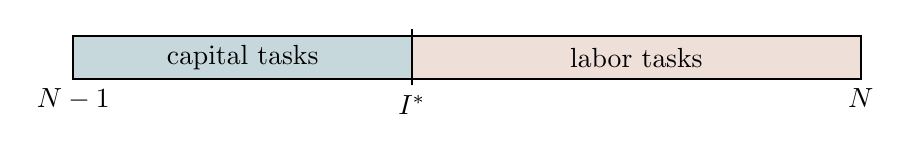
\begin{tikzpicture}[x=10.0cm,y=1cm]
\fill[accent!24] (0,0) rectangle (0.43,0.55);
\fill[warm!18] (0.43,0) rectangle (1,0.55);
\draw[thick] (0,0) rectangle (1,0.55);
\draw[thick] (0.43,-0.08)--(0.43,0.64);
\node[below] at (0,0) {$N-1$};\node[below] at (0.43,-0.08) {$I^*$};\node[below] at (1,0) {$N$};
\node at (0.215,0.27) {capital tasks};\node at (0.715,0.27) {labor tasks};
\end{tikzpicture}
\end{center}
\begin{itemize}
\item Automation moves the feasible frontier $I$ right; new tasks move $N$ right and replace the lowest tasks.
\item The measure of tasks stays one. The \key{composition} of that measure changes. At $\sigma=1$, use the continuous CES limit.
\end{itemize}
\sourcefoot
\end{frame}

\begin{frame}{The threshold is economic as well as technological}
\[
p(i)=\begin{cases}
\min\{R,\,W/\gamma(i)\},&i\leq I,\\
W/\gamma(i),&i>I,
\end{cases}
\qquad \frac{W}{R}=\gamma(\widetilde I),\qquad I^*=\min\{I,\widetilde I\}.
\]
\begin{itemize}\setlength\itemsep{0.55em}
\item $I$ says where capital \emph{can} perform a task; $\widetilde I$ says where it is \emph{cost effective}.
\item Strictly increasing $\gamma(i)$ gives labor comparative advantage at higher task indices.
\item If $I<\widetilde I$, technology binds. If $\widetilde I<I$, extra automation capacity has no immediate allocation effect.
\end{itemize}
\sourcefoot
\end{frame}

\begin{frame}{Two forces, two moving margins}
\begin{columns}[T,onlytextwidth]
\column{0.47\textwidth}
\key{Displacement: $I\uparrow$}\\[0.5em]
Capital takes tasks previously done by labor. Workers crowd into fewer tasks; relative labor demand and the labor share fall when the technology constraint binds.
\column{0.47\textwidth}
\key{Reinstatement: $N\uparrow$}\\[0.5em]
New, more complex tasks favor labor. The labor task range expands; relative demand, the labor share, and employment rise under the static assumptions.
\end{columns}
\vspace{0.85em}
\centering\large Both changes can raise productivity; the distributional signs differ.
\sourcefoot
\end{frame}

\begin{frame}{Static comparative statics need the conditions}
\small Proposition 2: Assumptions 1--3; $\varepsilon_L>0$; $\Lambda_I,\Lambda_N>0$; $K$ fixed.
\vspace{0.4em}
\begin{center}
\begin{tabular}{p{4.3cm}ccc}
\toprule
Regime and change & $W/R$ & labor share & employment \\
\midrule
$I^*=I<\widetilde I$, $dI>0$ & $-$ & $-$ & $-$ \\
$I^*=\widetilde I<I$, $dI>0$ & $0$ & $0$ & $0$ \\
Either regime, $dN>0$ & $+$ & $+$ & $+$ \\
\bottomrule
\end{tabular}
\end{center}
\[
\left.\frac{\partial\ln(W/R)}{\partial I}\right|_{I^*=I}
=-\frac{\Lambda_I}{\widehat\sigma+\varepsilon_L}<0,
\qquad
\left.\frac{\partial\ln(W/R)}{\partial N}\right|_{I^*=I}
=\frac{\Lambda_N}{\widehat\sigma+\varepsilon_L}>0.
\]
\sourcefoot
\end{frame}

\begin{frame}{Does automation necessarily lower wages? No}
\small Proposition 3, under Assumptions 1--3 and the \key{binding} threshold $I^*=I<\widetilde I$:
\[
\frac{\partial\ln W}{\partial I}
=\underbrace{\left.\frac{\partial\ln Y}{\partial I}\right|_{K,L}}_{P_I\;\text{productivity gain}}
-\underbrace{(1-s_L)\frac{\Lambda_I}{\widehat\sigma+\varepsilon_L}}_{D_I\;\text{displacement}}.
\]
\begin{center}
\fbox{\large $\displaystyle \frac{\partial\ln W}{\partial I}>0\quad\Longleftrightarrow\quad P_I>D_I$}
\end{center}
\begin{itemize}
\item The paper states a capital threshold: for sufficiently low $K$ (within Assumption 3), productivity dominates; at higher admissible $K$, displacement dominates.
\item If $I^*=\widetilde I<I$, raising feasible $I$ has \key{zero} marginal effect.
\end{itemize}
\sourcefoot
\end{frame}

\begin{frame}{An uncalibrated numerical sign check}
\small Hold $s_L=0.6$, $\Lambda_I=1$, $\widehat\sigma=1$, $\varepsilon_L=1$. Then $D_I=(1-0.6)/(1+1)=0.20$.
\vspace{0.7em}
\begin{center}
\begin{tabular}{ccc}
\toprule
Illustrative $P_I$ & $P_I-D_I$ & Wage response \\
\midrule
$0.05$ & $-0.15$ & falls \\
$0.20$ & $0$ & unchanged \\
$0.35$ & $+0.15$ & rises \\
\bottomrule
\end{tabular}
\end{center}
\vspace{0.5em}
These are \key{algebra checks}, not estimated model parameters. In all three binding cases, the relative wage $W/R$ and labor share still fall under Proposition 2.
\sourcefoot
\end{frame}

\begin{frame}{Long-run effects are different}
\small With exogenous technology and capital accumulation (Propositions 4--5), impose $\gamma(i)=e^{Ai}$ with $A>0$ (Assumption $1'$) and Assumption 2. On an interior BGP, $n=N-I\in(0,1)$ and $R=\rho+\delta+\theta g$.
\vspace{0.5em}
\begin{itemize}\setlength\itemsep{0.55em}
\item If $n>\bar n(\rho)$ and automation permanently reduces $n$, long-run employment and the labor share fall, while the \key{long-run wage rises} as capital adjusts.
\item If $n<\bar n(\rho)$, small increases in the automation frontier leave the equilibrium task allocation and effective wages unchanged.
\item The short-run wage may fall even when the long-run wage rises.
\end{itemize}
\sourcefoot
\end{frame}

\begin{frame}{Endogenous innovation: the main BGP result}
\small Proposition 6 requires Assumptions $1'$ ($\gamma=e^{Ai}, A>0$), 2 ($\eta\to0$ or $\zeta=1$), and 4 ($\widehat\sigma>\zeta$), plus sufficiently small scientist supply $S<\bar S$.
\vspace{0.35em}
\begin{center}
\begin{tabular}{p{4.2cm}p{7.1cm}}
\toprule
Condition & Balanced growth outcome \\
\midrule
$\rho<\bar\rho$ & A full-automation BGP exists: $n=0$, all tasks capital performed. \\
$\rho>\bar\rho$, $\kappa_N/\kappa_I>\bar\kappa$ & Unique interior BGP: $n\in(\bar n(\rho),1)$ and $\kappa_N v_N(n)=\kappa_I v_I(n)$. \\
$\rho>\bar\rho$, $\bar\kappa>\kappa_N/\kappa_I>\underline\kappa$ & Multiple BGPs. \\
$\rho>\bar\rho$, $\kappa_N/\kappa_I<\underline\kappa$ & Unique no-automation BGP: $n=1$; all tasks use labor. \\
\bottomrule
\end{tabular}
\end{center}
\scriptsize Here $\bar\rho=B-\delta-\theta g$ on a BGP; $\underline\kappa,\bar\kappa$ are the paper's innovation-ratio cutoffs. The equalities are separate boundary cases.
\sourcefoot
\end{frame}

\begin{frame}{Why the interior path can be stable}
\small In Proposition 6's unique interior case, $\kappa_I v_I(n)=\kappa_N v_N(n)$ with $n=N-I$. A fall in $n$ means automation has run ahead.
\vspace{0.7em}
\begin{itemize}\setlength\itemsep{0.65em}
\item A smaller $n$ makes producing with labor cheaper at the frontier, reducing the payoff to \emph{further} automation and supporting new task creation.
\item Stability additionally needs the relative value functions to cross with the correct slope; the paper's sufficient condition is $\kappa_N/\kappa_I>\bar\kappa$ and $S<\bar S$.
\item If $\theta=0$, equilibrium is globally saddle-path stable. If $\theta>0$, uniqueness and asymptotic saddle-path stability are local.
\end{itemize}
\sourcefoot
\end{frame}

\begin{frame}[fragile]{Lean slide: the cost threshold}
\small Original claim around equations (5)--(6):
\[
\frac{W}{R}=\gamma(\widetilde I),\quad I^*=\min\{I,\widetilde I\},\quad
 i<I^*\Rightarrow R<\frac{W}{\gamma(i)}.
\]
\begin{lstlisting}
def thresholdCostRankingSpec : Prop :=
  ∀ (γ : ℝ → ℝ) (w R I costThreshold : ℝ),
    StrictMono γ → (∀ i, 0 < γ i) → 0 < w → 0 < R →
    w / R = γ costThreshold →
      (∀ i, i < implementedThreshold I costThreshold →
        i ≤ I ∧ R < laborUnitCost w γ i) ∧
\end{lstlisting}
\begin{lstlisting}
have hγlt : γ i < γ costThreshold := hmono hiCost
have hmul : γ i * R < w := by
  apply (lt_div_iff₀ hR).mp
  rw [heq]
  exact hγlt
\end{lstlisting}
\scriptsize Lean assumes positive, strictly increasing $\gamma$ on all $\mathbb R$, stronger than the active task interval. \texttt{hmono hiCost} transfers task order to $\gamma$; \texttt{lt\_div\_iff\_0 hR} uses $R>0$. \key{Lean checks conditional cost ranking, not equilibrium existence.} Build passes; no \texttt{sorry}.
\end{frame}

\begin{frame}[fragile]{Lean slide: the wage sign and its boundary}
\small Proposition 3's constrained-case equation with $dN=0$ becomes:
\[
\partial_I\ln W=P_I-(1-s_L)\Lambda_I/(\widehat\sigma+\varepsilon_L).
\]
\begin{lstlisting}
noncomputable def automationWageResponse
    (productivityGain laborShare ΛI σhat εL : ℝ) : ℝ :=
  productivityGain - (1 - laborShare) * (ΛI / (σhat + εL))
\end{lstlisting}
\begin{lstlisting}
theorem automationWageSign : automationWageSignSpec := by
  intro productivityGain laborShare ΛI σhat εL _ _ _ _ _
  unfold automationWageResponse
  constructor <;> intro h <;> linarith
\end{lstlisting}
\small The final tactic proves the \emph{sign equivalence} once the response equation is supplied. It does not derive the equation or $P_I$ from production and market clearing. This is a \key{partial formalization} of Proposition 3. The paper-scoped fast check passed.
\end{frame}

\begin{frame}{Where I checked the AI myself}
\small The trap prompt was: \emph{``Does automation necessarily reduce wages and the labour share in this model?''}
\begin{columns}[T,onlytextwidth]
\column{0.55\textwidth}
\key{My derivation to photograph}
\[
\begin{aligned}
dN&=0,\ dI>0,\ I^*=I<\widetilde I,\\
\partial_I\ln W&=P_I-D_I,\\
D_I&=(1-s_L)\Lambda_I/(\widehat\sigma+\varepsilon_L),\\
\partial_I\ln W>0&\iff P_I>D_I.
\end{aligned}
\]
\column{0.42\textwidth}
\centering\IfFileExists{hand/derivation.jpg}{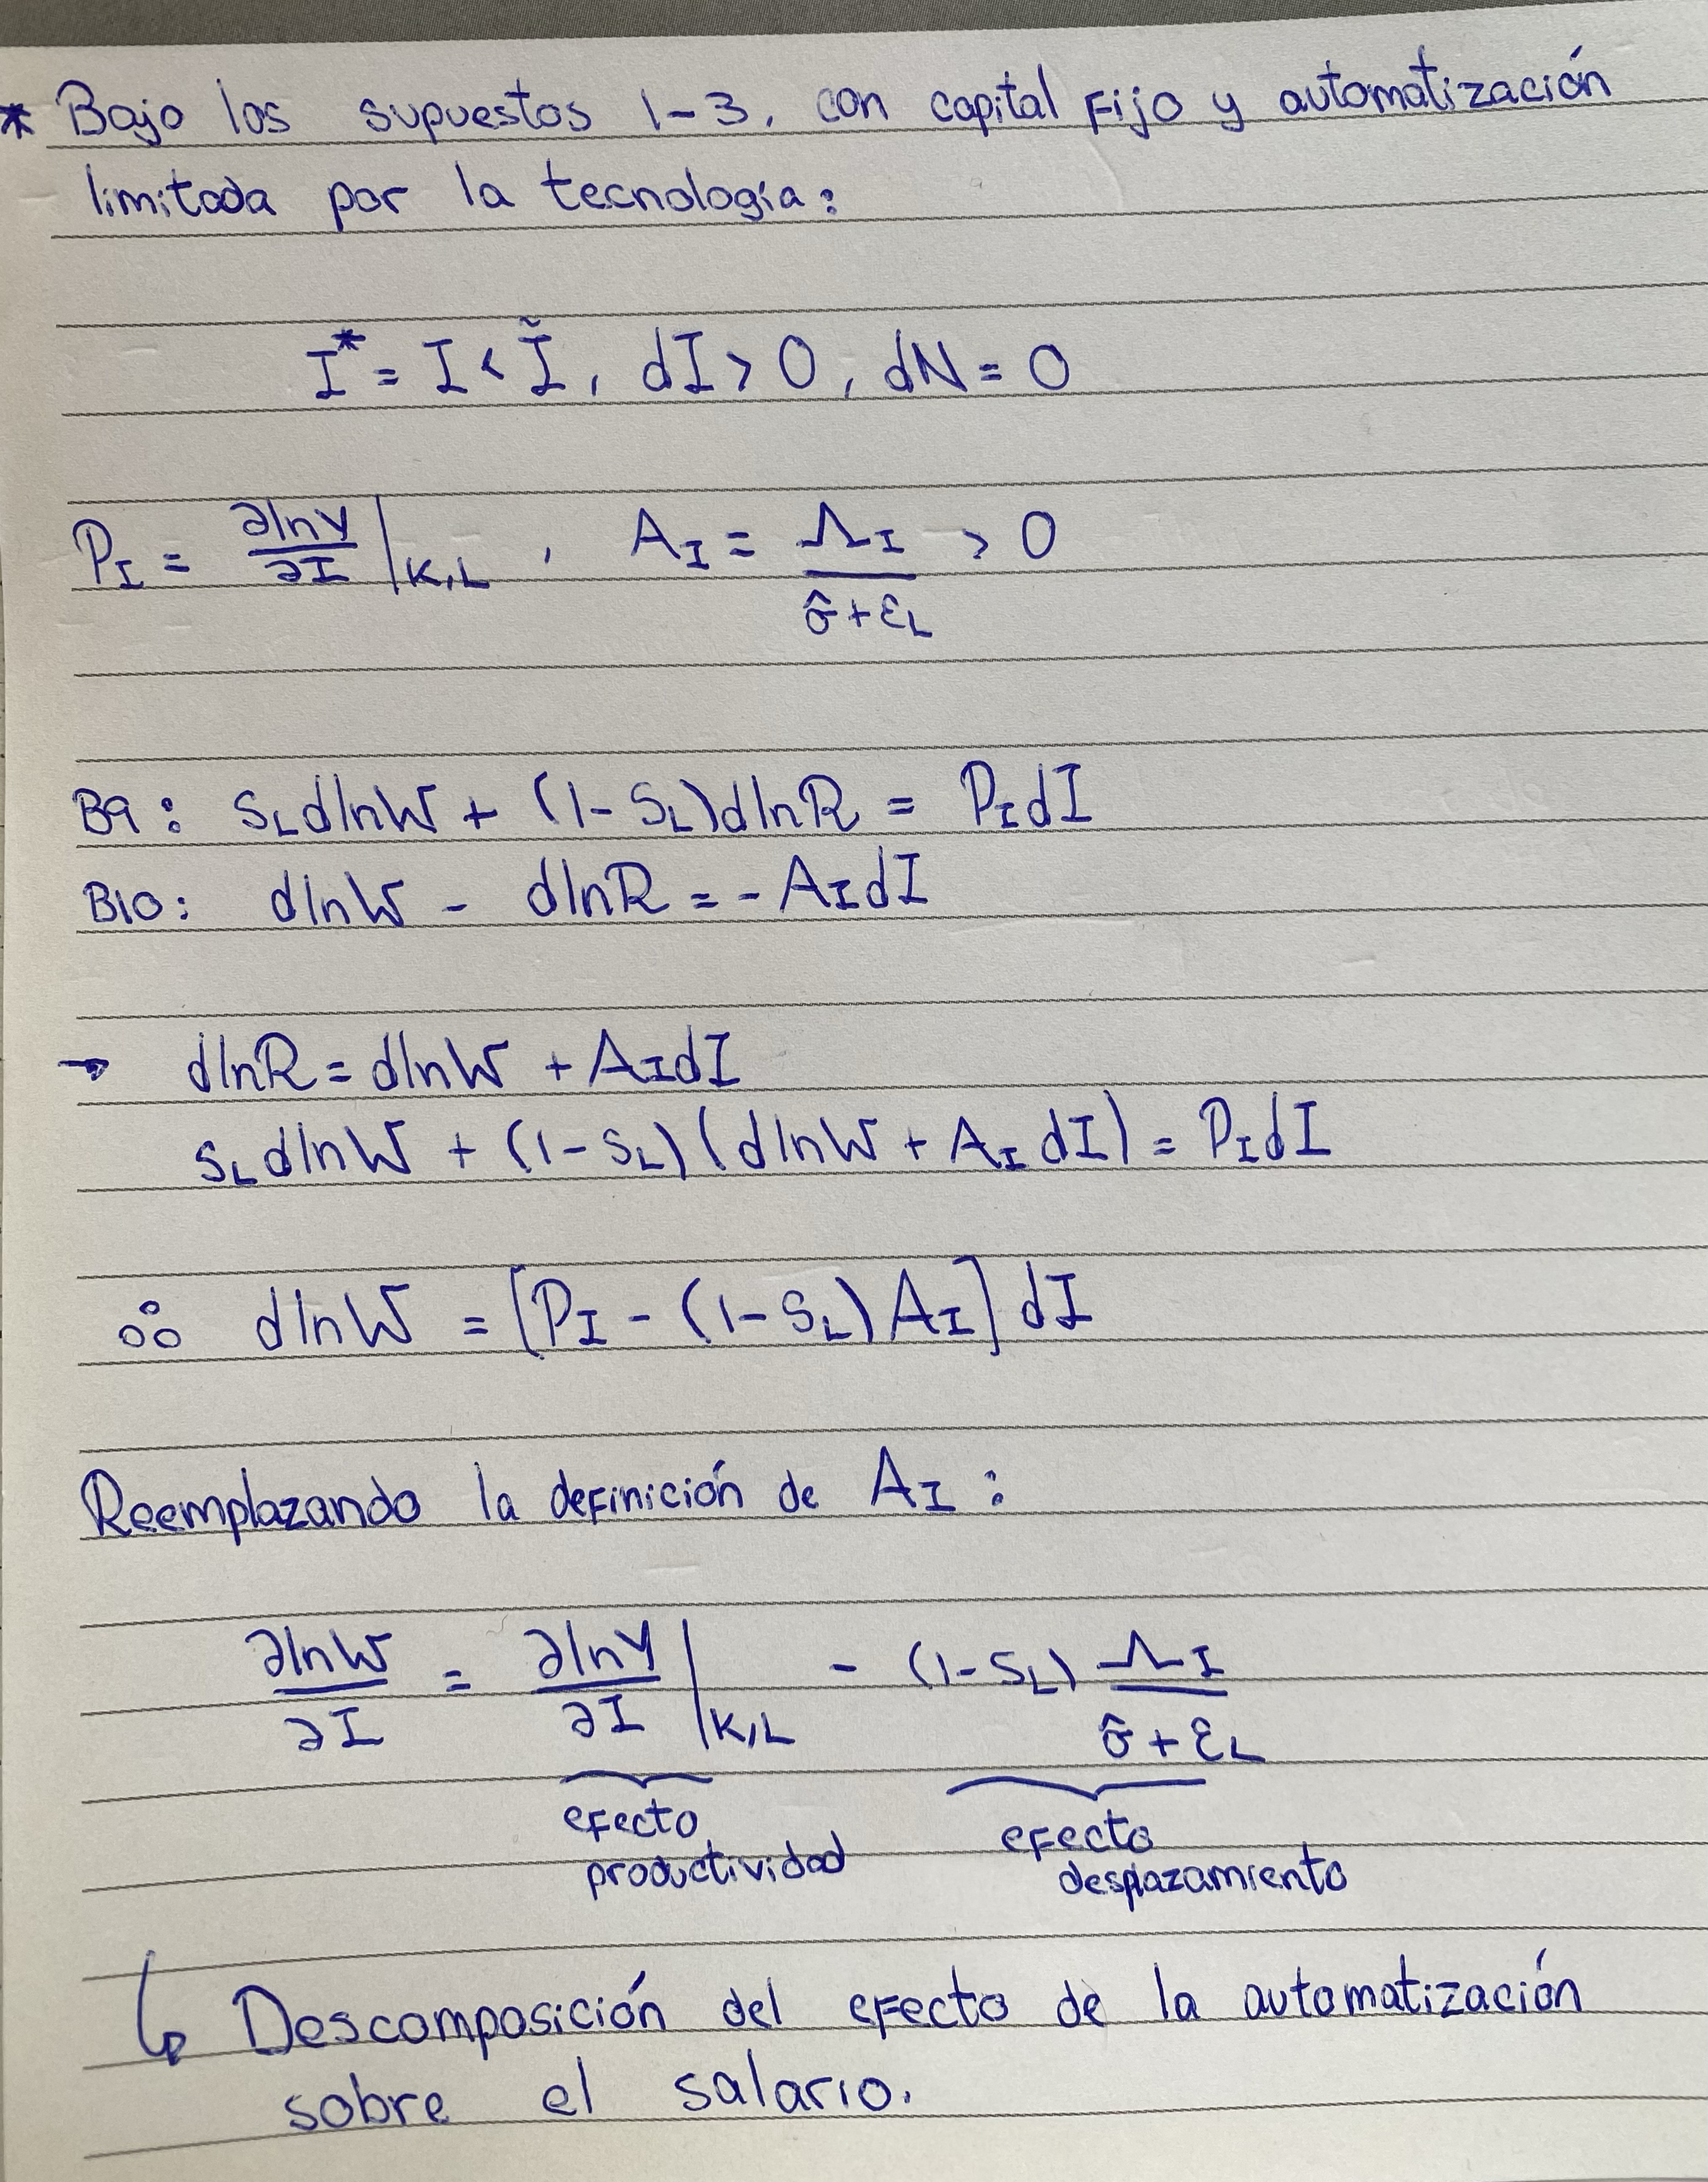
\includegraphics[width=\linewidth,height=3.0cm,keepaspectratio]{hand/derivation.jpg}}{\fbox{\parbox[c][2.1cm][c]{0.86\linewidth}{\centering Hand derivation photo pending\\Place at \texttt{hand/derivation.jpg}}}}
\end{columns}
\vspace{0.3em}\small \key{Verdict:} the flat claim ``automation lowers both'' is false for wages; and even the labor-share decrease requires an effective, binding expansion of automated tasks.
\sourcefoot
\end{frame}

\begin{frame}{What I did and what remains open}
\begin{columns}[T,onlytextwidth]
\column{0.48\textwidth}
\key{Analytical and computational work}
\begin{itemize}
\item Reconstructed the technology and cost thresholds.
\item Derived the wage sign condition.
\item Tested both signs with illustrative numbers.
\item Ran two Lean proofs and the paper-scoped fast check.
\end{itemize}
\column{0.48\textwidth}
\key{Translation boundary}
\begin{itemize}
\item No Lean proof of equilibrium existence or uniqueness.
\item No derivation of $P_I$, $\Lambda_I$, or the balanced growth conditions from primitives.
\item Full source-to-Lean semantic audit remains open; the generated folder records that status.
\end{itemize}
\end{columns}
\sourcefoot
\end{frame}

\begin{frame}{Takeaway}
\large Automation reallocates tasks to capital. New tasks reinstate labor at the frontier.
\vspace{0.7em}
\begin{itemize}\setlength\itemsep{0.7em}
\item Under the static model's assumptions, binding automation lowers relative wages, the labor share, and employment.
\item The \key{absolute wage} rises only when the productivity gain exceeds displacement; in the long run, capital adjustment can reverse a short-run wage decline.
\item Lean made the threshold, positive denominators, and proof boundary explicit. It verified a useful slice of the argument, not the whole equilibrium model.
\end{itemize}
\sourcefoot
\end{frame}

\end{document}
